\documentclass{beamer}
\usetheme{default}
\usecolortheme{dove}
\usepackage{amsmath,amssymb}
\usepackage{tikz}
\usetikzlibrary{arrows.meta,positioning,calc}

\setbeamertemplate{navigation symbols}{}
\setbeamertemplate{footline}[frame number]

\title{Why $\gamma$ Doesn't Learn:\\Centered vs.\ Non-Centered MAP}
\author{}
\date{}

\begin{document}

\begin{frame}
\titlepage
\end{frame}

%% ============================================================
%% SLIDE: How ML Training Works
%% ============================================================
\begin{frame}{How ML Training Works (4 Steps, Every Epoch)}

\begin{center}
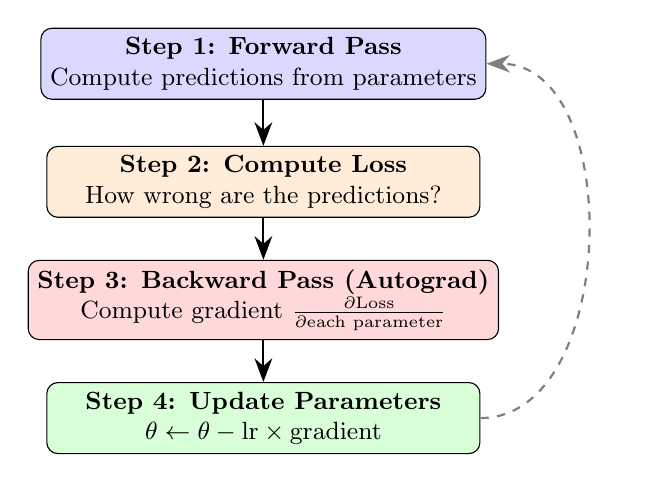
\begin{tikzpicture}[
    box/.style={rectangle, draw, rounded corners, minimum width=5.5cm, minimum height=0.9cm, font=\small, align=center},
    arr/.style={-{Stealth[length=3mm]}, thick}
]
    \node[box, fill=blue!15] (fwd) at (0,3) {\textbf{Step 1: Forward Pass}\\Compute predictions from parameters};
    \node[box, fill=orange!15] (loss) at (0,1.5) {\textbf{Step 2: Compute Loss}\\How wrong are the predictions?};
    \node[box, fill=red!15] (back) at (0,0) {\textbf{Step 3: Backward Pass (Autograd)}\\Compute gradient $\frac{\partial \text{Loss}}{\partial \text{each parameter}}$};
    \node[box, fill=green!15] (update) at (0,-1.5) {\textbf{Step 4: Update Parameters}\\$\theta \leftarrow \theta - \text{lr} \times \text{gradient}$};

    \draw[arr] (fwd) -- (loss);
    \draw[arr] (loss) -- (back);
    \draw[arr] (back) -- (update);
    \draw[arr, dashed, gray] (update.east) to[out=0,in=0] (fwd.east);
\end{tikzpicture}
\end{center}

\vspace{0.3cm}

\textbf{Key rule:} In Step 3, a parameter only gets a gradient from the loss if it was \textbf{used in Step 1} to compute the prediction. If a parameter isn't in the forward pass, autograd can't trace back to it.

\end{frame}

%% ============================================================
%% SLIDE: The Hierarchical Model
%% ============================================================
\begin{frame}{The Hierarchical Model}

\begin{center}
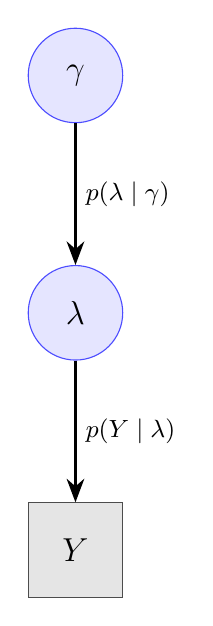
\begin{tikzpicture}[
    node distance=1.8cm,
    param/.style={circle, draw=blue!70, fill=blue!10, minimum size=1.2cm, font=\large},
    data/.style={rectangle, draw=black!70, fill=gray!20, minimum size=1.2cm, font=\large},
    arr/.style={-{Stealth[length=3mm]}, thick}
]
    \node[param] (gamma) {$\gamma$};
    \node[param, below=of gamma] (lambda) {$\lambda$};
    \node[data, below=of lambda] (Y) {$Y$};

    \draw[arr] (gamma) -- node[right, font=\small] {$p(\lambda \mid \gamma)$} (lambda);
    \draw[arr] (lambda) -- node[right, font=\small] {$p(Y \mid \lambda)$} (Y);
\end{tikzpicture}
\end{center}

\vspace{0.3cm}

\textbf{ALADYN:}
\begin{itemize}
    \item $\gamma$ = genetic effects on disease signatures (hyperparameter)
    \item $\lambda$ = individual latent trajectories (latent variable)
    \item $Y$ = observed disease diagnoses (data)
\end{itemize}

\vspace{0.3cm}
\textbf{Both models} have the same objective:
\[
\underset{\lambda,\, \gamma}{\text{minimize}} \;\; \underbrace{-\log p(Y \mid \lambda)}_{\text{NLL}} \;+\; \underbrace{-\log p(\lambda \mid \gamma)}_{\text{GP prior}}
\]

\end{frame}

%% ============================================================
%% SLIDE: The Centered Forward Pass
%% ============================================================
\begin{frame}{Centered Model: The Forward Pass}

\textbf{What the computer does each epoch:}

\vspace{0.4cm}

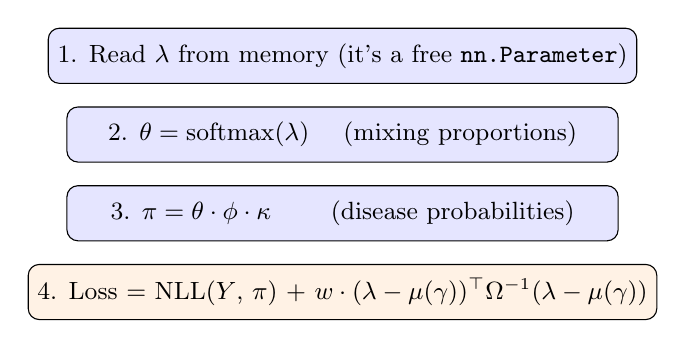
\begin{tikzpicture}[
    box/.style={rectangle, draw, rounded corners, minimum width=7cm, minimum height=0.7cm, font=\small, align=left},
]
    \node[box, fill=blue!10] (s1) at (0,3) {1. Read $\lambda$ from memory (it's a free \texttt{nn.Parameter})};
    \node[box, fill=blue!10] (s2) at (0,2) {2. $\theta = \text{softmax}(\lambda)$ \quad (mixing proportions)};
    \node[box, fill=blue!10] (s3) at (0,1) {3. $\pi = \theta \cdot \phi \cdot \kappa$ \quad\quad (disease probabilities)};
    \node[box, fill=orange!10] (s4) at (0,0) {4. Loss = NLL($Y$, $\pi$) + $w \cdot (\lambda - \mu(\gamma))^\top \Omega^{-1} (\lambda - \mu(\gamma))$};
\end{tikzpicture}

\vspace{0.5cm}

\textbf{Notice:} $\gamma$ appears \textbf{only in the prior term} (Step 4), never in the forward computation (Steps 1--3).

\vspace{0.3cm}

$\lambda$ is read from memory $\rightarrow$ $\theta$ $\rightarrow$ $\pi$ $\rightarrow$ NLL. \\
The chain $Y \rightarrow \pi \rightarrow \theta \rightarrow \lambda$ does not pass through $\gamma$.

\end{frame}

%% ============================================================
%% SLIDE: The Reparam Forward Pass
%% ============================================================
\begin{frame}{Reparameterized Model: The Forward Pass}

\textbf{What the computer does each epoch:}

\vspace{0.4cm}

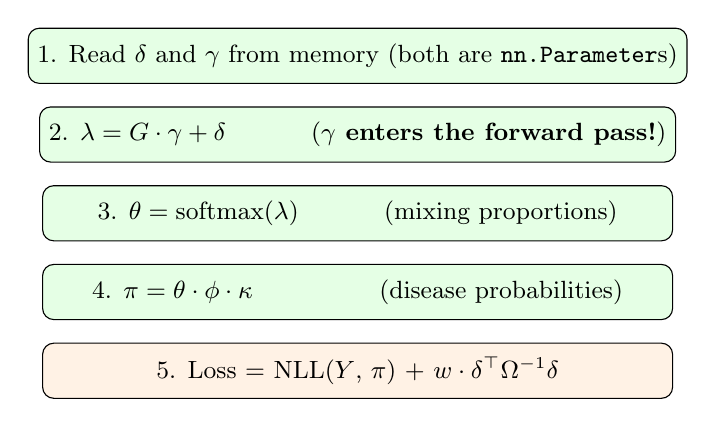
\begin{tikzpicture}[
    box/.style={rectangle, draw, rounded corners, minimum width=8cm, minimum height=0.7cm, font=\small, align=left},
]
    \node[box, fill=green!10] (s1) at (0,3) {1. Read $\delta$ and $\gamma$ from memory (both are \texttt{nn.Parameter}s)};
    \node[box, fill=green!10] (s2) at (0,2) {2. $\lambda = G \cdot \gamma + \delta$ \quad\quad\quad (\textbf{$\gamma$ enters the forward pass!})};
    \node[box, fill=green!10] (s3) at (0,1) {3. $\theta = \text{softmax}(\lambda)$ \quad\quad\quad (mixing proportions)};
    \node[box, fill=green!10] (s4) at (0,0) {4. $\pi = \theta \cdot \phi \cdot \kappa$ \quad\quad\quad\quad\; (disease probabilities)};
    \node[box, fill=orange!10] (s5) at (0,-1) {5. Loss = NLL($Y$, $\pi$) + $w \cdot \delta^\top \Omega^{-1} \delta$};
\end{tikzpicture}

\vspace{0.5cm}

\textbf{Now:} $\gamma$ is \textbf{in the forward computation} (Step 2). \\
The chain is: $\gamma \rightarrow \lambda \rightarrow \theta \rightarrow \pi \rightarrow$ NLL.

\vspace{0.3cm}

Autograd traces back through this chain, so $\gamma$ gets a gradient from the data.

\end{frame}

%% ============================================================
%% SLIDE: The Backward Pass — Why Gamma Gets Left Out
%% ============================================================
\begin{frame}{The Backward Pass: Why $\gamma$ Gets Left Out}

\textbf{Centered model} --- backward pass computes:

\[
\frac{\partial \text{Loss}}{\partial \lambda} = \underbrace{\frac{\partial \text{NLL}}{\partial \lambda}}_{\text{\color{green!60!black} data signal (strong)}} + \underbrace{w \cdot \frac{\partial \text{prior}}{\partial \lambda}}_{\text{\color{blue} prior signal (weak)}}
\]

\[
\frac{\partial \text{Loss}}{\partial \gamma} = \underbrace{\overset{{\color{red}\mathbf{= 0}}}{\frac{\partial \text{NLL}}{\partial \gamma}}}_{\text{\color{red} Not in forward pass!}} + \underbrace{w \cdot \frac{\partial \text{prior}}{\partial \gamma}}_{\text{\color{blue} prior only ($w$=1e-4)}}
\]

\pause
\vspace{0.3cm}
\hrule
\vspace{0.3cm}

\textbf{Reparam model} --- backward pass computes:

\[
\frac{\partial \text{Loss}}{\partial \gamma} = \underbrace{\frac{\partial \text{NLL}}{\partial \pi} \cdot \frac{\partial \pi}{\partial \theta} \cdot \frac{\partial \theta}{\partial \lambda} \cdot \frac{\partial \lambda}{\partial \gamma}}_{\text{\color{green!60!black} chain rule through forward pass!}} + \; 0
\]

$\gamma$ \textbf{is in the forward pass}, so the NLL gradient flows back to it.

\end{frame}

%% ============================================================
%% SLIDE: Same Objective, Different Computation
%% ============================================================
\begin{frame}{Same Objective, Different Computation}

Both models minimize the \textbf{same function}:
\[
p(Y \mid \lambda) \cdot p(\lambda \mid \gamma)
\]

\pause
\vspace{0.2cm}

The difference is purely in \textbf{how the computer represents $\lambda$}:

\vspace{0.3cm}

\begin{tabular}{l|c|c}
 & \textbf{Centered} & \textbf{Non-centered (Reparam)} \\ \hline
\rule{0pt}{2.5ex}Free parameters & $\lambda$, $\gamma$ & $\delta$, $\gamma$ \\[4pt]
Forward pass & $\theta = \text{softmax}(\lambda)$ & $\lambda = G\gamma + \delta$ \\
 & & $\theta = \text{softmax}(\lambda)$ \\[4pt]
NLL & $-\log p(Y \mid \lambda)$ & $-\log p(Y \mid G\gamma + \delta)$ \\[4pt]
Prior & \multicolumn{2}{c}{$(\lambda - G\gamma)^\top \Omega^{-1} (\lambda - G\gamma) \;=\; \delta^\top \Omega^{-1} \delta$ \quad (identical)} \\[4pt]
$\gamma$ in NLL? & \color{red}{No} & \color{green!60!black}{Yes} \\[2pt]
$\gamma$ gets data grad? & \color{red}{No} & \color{green!60!black}{Yes} \\
\end{tabular}

\vspace{0.5cm}
\textbf{At any solution:} $\delta^* = \lambda^* - G\gamma^*$. If the problem were convex, both would find the same optimum. Because it is \textbf{non-convex}, different gradient flows $\rightarrow$ different local optima.

\end{frame}

%% ============================================================
%% SLIDE: The Gradient Flow Picture
%% ============================================================
\begin{frame}{The Gradient Flow Picture}

\begin{columns}
\column{0.48\textwidth}
\textbf{Centered:}
\begin{center}
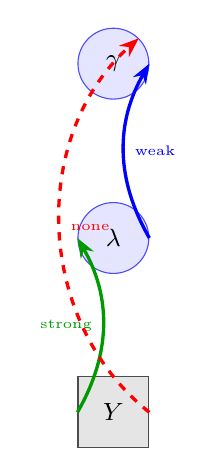
\begin{tikzpicture}[
    node distance=1.3cm,
    param/.style={circle, draw=blue!70, fill=blue!10, minimum size=0.9cm, font=\small},
    data/.style={rectangle, draw=black!70, fill=gray!20, minimum size=0.9cm, font=\small},
    grad/.style={-{Stealth[length=2.5mm]}, very thick},
]
    \node[param] (gamma) {$\gamma$};
    \node[param, below=of gamma] (lambda) {$\lambda$};
    \node[data, below=of lambda] (Y) {$Y$};

    \draw[grad, green!60!black] (Y.west) to[bend right=30] node[left, font=\tiny, text=green!60!black] {strong} (lambda.west);
    \draw[grad, blue] (lambda.east) to[bend left=30] node[right, font=\tiny, text=blue] {weak} (gamma.east);
    \draw[grad, red, dashed] (Y.east) to[bend left=50] node[right, font=\tiny, text=red] {none} (gamma.north east);
\end{tikzpicture}
\end{center}

\column{0.48\textwidth}
\textbf{Non-centered:}
\begin{center}
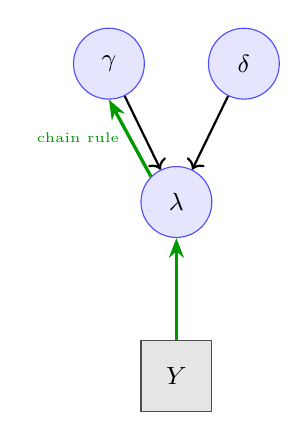
\begin{tikzpicture}[
    node distance=1.3cm,
    param/.style={circle, draw=blue!70, fill=blue!10, minimum size=0.9cm, font=\small},
    data/.style={rectangle, draw=black!70, fill=gray!20, minimum size=0.9cm, font=\small},
    grad/.style={-{Stealth[length=2.5mm]}, very thick},
]
    \node[param] (gamma) {$\gamma$};
    \node[param, right=0.8cm of gamma] (delta) {$\delta$};
    \node[param, below=1.3cm of $(gamma)!0.5!(delta)$] (lambda) {$\lambda$};
    \node[data, below=of lambda] (Y) {$Y$};

    \draw[thick, ->] (gamma) -- (lambda);
    \draw[thick, ->] (delta) -- (lambda);
    \draw[grad, green!60!black] (Y) -- (lambda);
    \draw[grad, green!60!black] (lambda.north west) -- node[left, font=\tiny, text=green!60!black] {chain rule} (gamma.south);
\end{tikzpicture}
\end{center}
\end{columns}

\vspace{0.5cm}

Both $\gamma$ and $\delta$ feed into $\lambda$ in the forward pass $\rightarrow$ both get NLL gradients.

In centered, $\lambda$ is a dead-end: gradients stop there and never reach $\gamma$ through the NLL.

\end{frame}

%% ============================================================
%% SLIDE: A Simple Analogy
%% ============================================================
\begin{frame}{A Simple Analogy}

Minimize $f(x) = (x - 3)^2$ with a preference that $x$ be near $\mu$:

\vspace{0.3cm}

\textbf{Centered:}
\begin{itemize}
    \item Parameters: $x$ and $\mu$
    \item Loss $= (x-3)^2 + w \cdot (x - \mu)^2$
    \item $\mu$ only appears in the penalty. If $w$ is small, $\mu$ barely moves.
\end{itemize}

\vspace{0.3cm}

\textbf{Non-centered:}
\begin{itemize}
    \item Parameters: $z$ and $\mu$, where $x = \mu + z$
    \item Loss $= (\mu + z - 3)^2 + w \cdot z^2$
    \item $\mu$ appears in the \textbf{main loss}. It gets a strong gradient.
\end{itemize}

\vspace{0.3cm}

Same answer ($x^* = 3$), but in the second form $\mu$ learns where $x$ wants to be. In the first form, $\mu$ barely moves because $w$ is tiny.

\end{frame}

%% ============================================================
%% SLIDE: Why It Usually Doesn't Matter
%% ============================================================
\begin{frame}{Why It Usually Doesn't Matter (for Prediction)}

$\lambda$ \textbf{compensates.}

\vspace{0.3cm}

For prediction, we:
\begin{enumerate}
    \item Fix all population parameters ($\phi, \gamma, \psi, \kappa$) from training
    \item For each new individual: re-estimate $\lambda_{\text{new}}$ (200 epochs)
    \item $\lambda_{\text{new}}$ has $K \times T$ free parameters --- enough to absorb the signal
\end{enumerate}

\vspace{0.3cm}

So even if $\gamma \approx 0$ (centered), $\lambda_{\text{new}}$ can still fit the data well.

\vspace{0.3cm}
\pause

\textbf{However}, it does still matter because:
\begin{itemize}
    \item Reparam initializes $\lambda = G\gamma + \delta$ (starting near the genetic prediction)
    \item Centered initializes $\lambda$ near zero (no genetic information at start)
    \item Different starting points $\rightarrow$ different optimization paths $\rightarrow$ different final $\lambda$
    \item Different trained $\phi/\psi/\kappa$ between the two pipelines also contribute
\end{itemize}

\end{frame}

%% ============================================================
%% SLIDE: Prediction Comparison
%% ============================================================
\begin{frame}{Prediction AUC: Centered vs.\ Non-Centered}

\small
50,000 held-out patients, 100 bootstrap replicates, 28 diseases:

\vspace{0.3cm}

\begin{center}
\begin{tabular}{l|c|c|c|c}
\textbf{Metric} & \textbf{Centered} & \textbf{Non-centered} & \textbf{$\Delta$} & \textbf{Wins} \\ \hline
\rule{0pt}{2.5ex}Static 10-year & 0.622 & 0.654 & +0.032 & 25/28 \\
Dynamic 10-year & 0.624 & 0.629 & +0.005 & 18/28 \\
Dynamic 1-year & 0.765 & 0.883 & +0.118 & 24/28 \\
\end{tabular}
\end{center}

\vspace{0.3cm}

\textbf{Non-centered wins on all 3 metrics.}

\vspace{0.2cm}

\begin{itemize}
    \item Largest advantage at short horizon (1-year: $+0.118$)
    \item Smallest advantage at dynamic 10-year ($+0.005$)
    \item \textbf{Caveat:} confounded by different population parameters ($\phi$, $\psi$, $\kappa$) between the two training pipelines --- not purely a parameterization effect
\end{itemize}

\end{frame}

%% ============================================================
%% SLIDE: Empirical Evidence - Parameter Differences
%% ============================================================
\begin{frame}{Trained Parameter Differences}

\begin{center}
\begin{tabular}{l|c|c}
 & \textbf{Centered} & \textbf{Non-centered} \\ \hline
\rule{0pt}{2.5ex}Mean $|\gamma|$ & 0.006 & 0.081 \\
$\kappa$ & 2.93 & 4.52 \\
$\gamma$ correlation & \multicolumn{2}{c}{0.37 (very different)} \\
$\psi$ correlation & \multicolumn{2}{c}{0.76 (moderately different)} \\
$\phi$ correlation & \multicolumn{2}{c}{0.94 (similar)} \\
\end{tabular}
\end{center}

\vspace{0.5cm}

\begin{itemize}
    \item $\phi$ (disease trajectories): nearly identical --- both fit the data well
    \item $\psi$ (signature assignments): moderately different --- non-centered less stable
    \item $\gamma$ (genetic effects): \textbf{centered $\gamma \approx 0$} (14$\times$ smaller)
    \item[]
    \item The \textbf{prediction AUC difference is driven by all of these} (especially $\phi$/$\psi$/$\kappa$), not just $\gamma$
\end{itemize}

\end{frame}

%% ============================================================
%% SLIDE: Summary
%% ============================================================
\begin{frame}{Summary}

\begin{enumerate}
    \item \textbf{ML training = forward $\rightarrow$ loss $\rightarrow$ backward $\rightarrow$ update.} A parameter only gets a data gradient if it was in the forward pass.

    \vspace{0.2cm}

    \item Both models optimize the same posterior: $p(Y|\lambda) \cdot p(\lambda|\gamma)$. \\
    The difference is whether you write $\lambda = G\gamma + \delta$ in the forward step.

    \vspace{0.2cm}

    \item \textbf{Centered} (original): $\lambda$ is free, $\gamma$ only in the prior $\rightarrow$ $\gamma$ gets no data gradient.

    \vspace{0.2cm}

    \item \textbf{Non-centered} (reparam): $\lambda = G\gamma + \delta$, $\gamma$ in forward pass $\rightarrow$ $\gamma$ gets data gradient via chain rule.

    \vspace{0.2cm}

    \item Both are standard approaches. Centered is the default in Stan/lme4/PyMC. Non-centered is the standard alternative.

    \vspace{0.2cm}

    \item For prediction: non-centered wins on AUC (all 3 metrics), but confounded by different population parameters.
\end{enumerate}

\end{frame}

\end{document}
